\documentclass[10pt,twocolumn]{article}

\usepackage[english]{babel}
\usepackage{amssymb}
\usepackage{amsmath}
\usepackage[left=1.5cm, right=1.5cm]{geometry}
\usepackage{csquotes}
\usepackage{caption}
\usepackage{graphicx}
\usepackage{multicol}
\usepackage[backend=biber]{biblatex}
\addbibresource{references.bib}
\graphicspath{ {./images/} }


\begin{document}

\title{Computational Neuroscience: \\ Inhibitory-Stabilised Networks}
\author{B204511}
\date{November 2024}
\maketitle

\section{Introduction}
Several brain regions, including the neocortex and hippocampus \cite{tsodyks1997paradoxical}
contain local recurrently connected networks of excitatory and inhibitory neurons.
Understanding how those networks function and react to external inputs is important
for analysing how the brain operates. This report will introduce the concept of
such networks, discuss their biological relevance, present a mathematical model, and provide
computer simulations as well as mathematical analysis of the model.

The network is viewed as consisting of 2 pools of neurons: excitatory and inhibitory.
Each pool projects to the other, and to itself, forming a recurrent neural network.
Excitatory feedback can lead to runaway excitation, which is prevented by the inhibitory feedback. 
This allows the network to stabilise, earning it the name Inhibitory-Stabilised Network (ISN).


To understand how the system comes together, it is important to get a sense of what 
the underlying model of each individual nueron is and how the interaction between them integrates.

% #######################
% Model of the Neuron
% #######################

\subsection{Leaky Integrate-and-Fire Neuron}
In 1907, Louis Édouard Lapicque \cite{brunel2007quantitative} introduced 
the concept of the integrate-and-fire neuron model.
Even though the model was developed before scientists 
had a chance to describe the biophysical mechanics of the neuron, 
it captured the behaviour of the neuron in a way that was useful 
for understanding \cite{abbott1999lapicque}.

The neuron is viewed as an electric circuit with a capacitor and a resistor connected in parallel.
% resistor
The membrane has some resistance, which is assumed to be constant and can be described by Ohm's law: $V = IR$, and therefore 
the resistor current is $I = \frac{V}{R} = gV$, where $g$ is conductance of the cell. 
% capacitor
The relationship between the current and the voltage across the capacitor is described by the following equation: 
$C = \frac{Q}{V}$, where $C$ is the capacitance, $Q$ is the charge stored in the capacitor, and $V$ is the voltage across the capacitor.
Knowing this, the current in the circuit: 

$$
I = \frac{dQ}{dt} = \frac{dCV}{dt} = C \frac{dV}{dt}
$$
% Combining the two, we get: $C \frac{dV}{dt} = gV$.

Real neurons, however, receive current from other neurons via dendrites from synapses,
and induce own \textbf{ionic} current by
% opening and closing ion channels (each with its own conductance) and 
letting charged particles 
% ($Na^+, Cl^-, Ca^{2+}, K^+$) 
in and out of the cell. Therefore,
the total current is the sum of the ionic current plus any external input: $I = \sum_{i}g_iV + I_{ext} = g_mV + I_{ext}$.
Neurons are generally \textbf{negatively charged} relative to the outside, and therefore the flow outside the cell is treated as positive.
Since the size of the cell and its channels is comparable to that of ions, effect of electric attraction is comparable with that of diffusion,
and there exists a point, where one balances out the other, resulting in the zero net current flow. 
This point is called the resting potential $V_{rest}$ of the neuron, and therefore any current should be measured relative to this potential.
 
$$
C \frac{dV}{dt} = -g_m(V - V_{\text{rest}}) + I_{\text{ext}}
$$

Dividing by conductance, we get the following equation:
$$
\tau_m \frac{dV}{dt} = -(V - V_{\text{rest}}) + \frac{I_{\text{ext}}}{g_m}
$$
where $\tau_m$ is the membrane time constant, describing how quickly it reacts to input.

Now, the external current is the component of interest,
by extending this component, we can integrate input from other neurons.
Neurons communicate by sending electrical signals to each other, via the synapse of 
emitting through the dendrites of the receiving neuron.
This interaction can be modelled as a synpatic current, weighted by the strength of connection. 
Dale's Law\cite{efron1968psychopharmacology} states that a neuron can only be 
either excitatory or inhibitory, and therefore we can simplify the model, and 
approximate the synaptic current as a function of emitting neuron's voltage:
$I_{\text{syn},i} = W\phi(V_i)$,
where $W$ is the synaptic weight ($+$ for excitatory, $-$ for inhibitory), and $\phi(V)$ is the transfer function of the neuron.
The actual external current collapses into $I_{ext}/g_m=u_{ext}$.

Combing all component, we obtain a system of equations:
\begin{equation}
    \tau_E \frac{dV_E}{dt} = 
    -(V_E - V_{\text{rest}}) 
    + W_{EE} \phi(V_E) 
    - W_{EI} \phi(V_I) + u_E
\end{equation}

\begin{equation}
    \tau_I \frac{dV_I}{dt} = 
    -(V_I - V_{\text{rest}}) 
    + W_{IE} \phi(V_E) 
    - W_{II} \phi(V_I) + u_I
\end{equation}
where $V_{\text{rest}}$ is the resting potential of the neuron, $W_{k}$ are the 
synaptic weights, $u_k$ are the external inputs to neurons, 
and $\phi(V)$ is the transfer function of a neuron, that acts as 
a communication channel between the neurons and is defined as a scaled ReLU function:

\begin{equation}
    \phi(V) = \beta[V-V_0]_+
\end{equation}

Now that we have the model and its origins, it's important to outline 
the benefits and limitations of the model.

\subsection{Considerations}
1. The model abstracts away certain biological complexity, such as stochasticity and
variability of individual ion channels (both in somas and synapses), described in
great detail by the Hodgkin-Huxley model \cite{hodgkin1952quantitative}, which is
a more biologically plausible model of the neuron, 
but is also signficantly more complex.

2. Synaptic weights are assumed to be constant, whereas in reality they are subject to
plasticity, and can change over time.
The weights themeselves are a heuristic approximation, 
by making which we sacrifice details of 
spiking patterns assuming them to be a linear function of the voltage.

3. The membrane time constant that comes from conductance is assumed to be constant,
and relies on Ohm's law, which is a simplification of the actual behaviour of the neuron.
However, it is a good approximation for the passive dynamics of a neuron.  

4. The LIF model is a lot more computationally affordable, requires 4 ODEs
per neuron in the HH model, instead of 1 in the LIF model, 
which allows us to run large scale simulations and analyse 
the network behaviour faster. The model is also more amenable 
to theoretic analysis, which helps to explain certain activity patterns in the network.

In essence, we trade off biological accuracy for 
computational efficiency and analytic tractability.


% ####################### 
% COMPUTER SIMULATIONS
% #######################

\section{Computer Simulations}
In this section, simulations of the network are presented,
where the network is stimulated with various external inputs for 
both excitatory and inhibitory pools, and the
response of the network is approximated numerically using the Euler method.

In our simulations, we study 2 networks with the following base parameters:
% V_rest
$$
V_{\text{rest}} = -70 \text{mV, } V_0 = -55 \text{mV, } \beta = 1
$$

% tau
$$
\tau 
= \begin{pmatrix} \tau_E \\ \tau_I \end{pmatrix} 
= \begin{pmatrix} 20 \\ 10 \end{pmatrix}\text{ms} 
$$

% Us
$$
u
= \begin{pmatrix} u_E \\ u_I \end{pmatrix}
= \begin{pmatrix} 20 \\ 20 \end{pmatrix}
$$

% Ws
$$
W 
= \begin{pmatrix} W_{EE} & W_{EI} \\ W_{IE} & W_{II} \end{pmatrix}
= \begin{pmatrix} W^n_{EE} & 0.65 \\ 1.2 & 0.5 \end{pmatrix}
$$

Where $W^n_{EE}$ is the weight of the excitatory feedback for a given network.
The 2 networks differ in the weight of the excitatory feedback, where one is weaker 
is $W^1_{EE} = 0.5$ and the other is stronger $W^2_{EE} = 1.25$.

\subsection{Stable External Input}
We first study both networks with a stable external input of 20mV to both neurons.
Both neurons start from the resting potential. The simulation is ran for 500ms 
with 1ms time steps. The results are shown in Figure \ref{fig:stable-input}.

Looking at the results for network 1 (solid lines), we can see that both neurons
gradually begin responding to the external input, and at some point begin firing

\begin{figure*}
    \centering
    \captionsetup{justification=centering}
    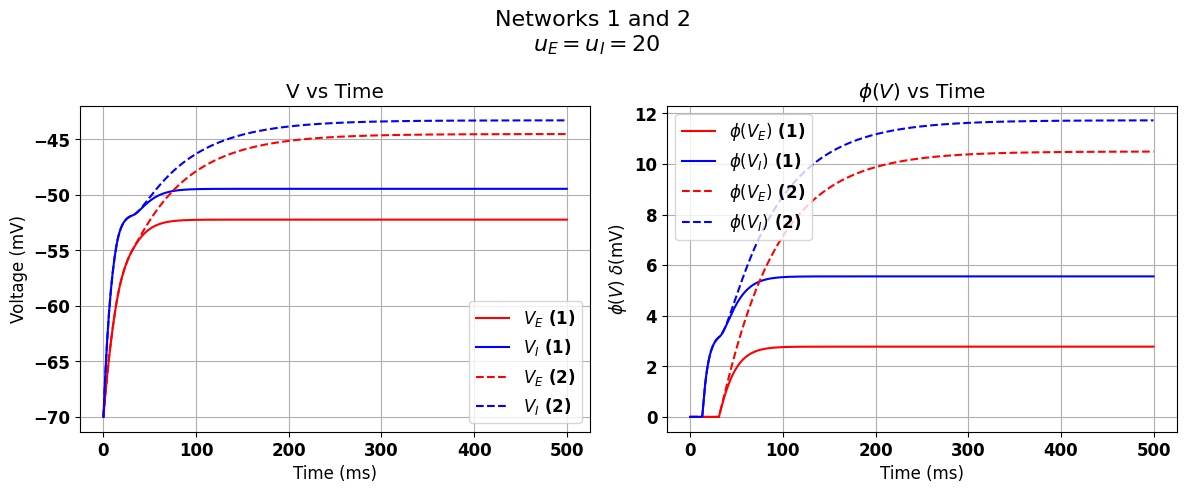
\includegraphics[width=1\textwidth]{images/12-stable.png}
    \caption{\textbf{Stable} external input to both neurons.\\ Excitatory potentials are red, inhibitory potentials are blue. \\Network 1 is solid, Network 2 is dashed.}
    \label{fig:stable-input}
\end{figure*}

\subsection{External Inhibitory Input Increase}


\begin{figure*}
    \centering
    \captionsetup{justification=centering}
    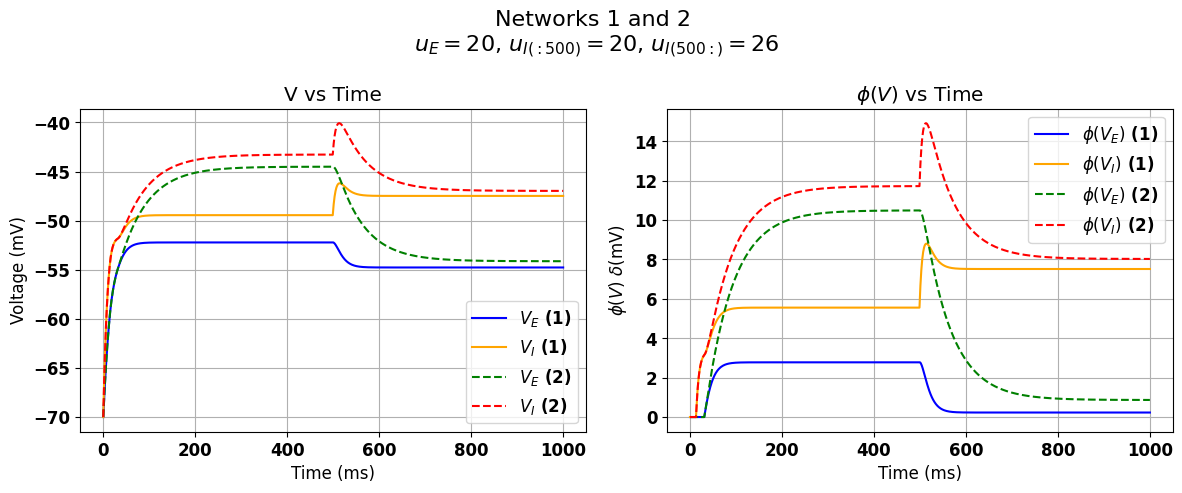
\includegraphics[width=1\textwidth]{images/12-I_input.png}
    \caption{External \textbf{inhibitory} input increase after 500ms. \\Excitatory potentials are red, inhibitory potentials are blue.\\Network 1 is solid, Network 2 is dashed.}
    \label{fig:i-input}
\end{figure*}

\begin{figure*}
    \centering
    \captionsetup{justification=centering}
    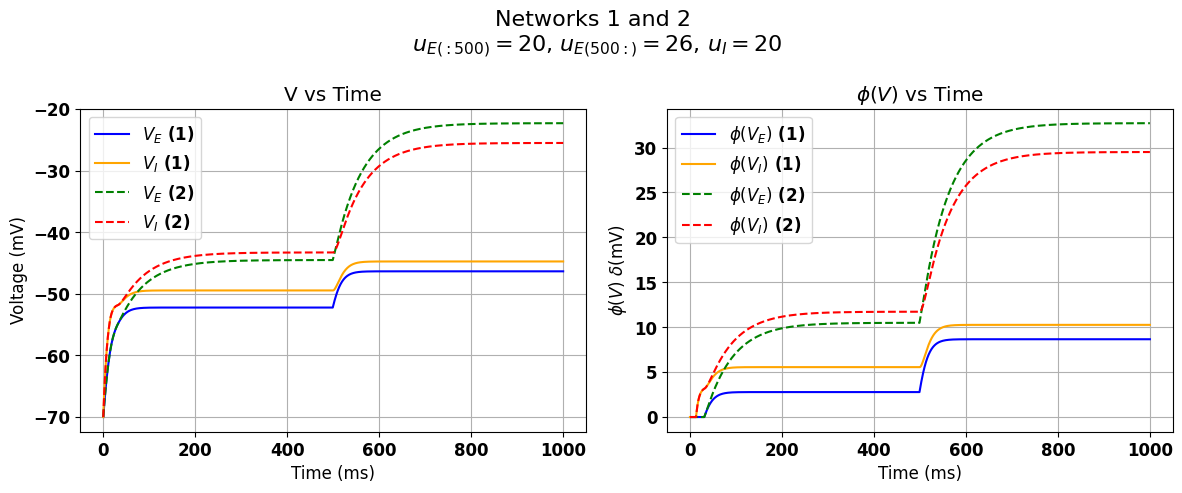
\includegraphics[width=1\textwidth]{images/12-E_input.png}
    \caption{External \textbf{excitatory} input increase after 500ms. Excitatory potentials are red, inhibitory potentials are blue.\\Network 1 is solid, Network 2 is dashed.}
    \label{fig:e-input}
\end{figure*}

\section{Mathematical Analysis}

\section{Conclusion}

\pagebreak
\printbibliography

\end{document}


